\documentclass[journal,12pt,twocolumn]{IEEEtran}

\usepackage{setspace}
\usepackage{gensymb}

\singlespacing


\usepackage[cmex10]{amsmath}

\usepackage{amsthm}

\usepackage{mathrsfs}
\usepackage{txfonts}
\usepackage{stfloats}
\usepackage{bm}
\usepackage{cite}
\usepackage{cases}
\usepackage{subfig}

\usepackage{longtable}
\usepackage{multirow}

\usepackage{enumitem}
\usepackage{mathtools}
\usepackage{steinmetz}
\usepackage{tikz}
\usepackage{circuitikz}
\usepackage{verbatim}
\usepackage{tfrupee}
\usepackage[breaklinks=true]{hyperref}
\usepackage{graphicx}
\usepackage{tkz-euclide}
\usepackage{float}

\usetikzlibrary{calc,math}
\usepackage{listings}
    \usepackage{color}                                            %%
    \usepackage{array}                                            %%
    \usepackage{longtable}                                        %%
    \usepackage{calc}                                             %%
    \usepackage{multirow}                                         %%
    \usepackage{hhline}                                           %%
    \usepackage{ifthen}                                           %%
    \usepackage{lscape}     
\usepackage{multicol}
\usepackage{chngcntr}

\DeclareMathOperator*{\Res}{Res}

\renewcommand\thesection{\arabic{section}}
\renewcommand\thesubsection{\thesection.\arabic{subsection}}
\renewcommand\thesubsubsection{\thesubsection.\arabic{subsubsection}}

\renewcommand\thesectiondis{\arabic{section}}
\renewcommand\thesubsectiondis{\thesectiondis.\arabic{subsection}}
\renewcommand\thesubsubsectiondis{\thesubsectiondis.\arabic{subsubsection}}


\hyphenation{op-tical net-works semi-conduc-tor}
\def\inputGnumericTable{}                                 %%

\lstset{
%language=C,
frame=single, 
breaklines=true,
columns=fullflexible
}
\begin{document}
\newtheorem{theorem}{Theorem}[section]
\newtheorem{problem}{Problem}
\newtheorem{proposition}{Proposition}[section]
\newtheorem{lemma}{Lemma}[section]
\newtheorem{corollary}[theorem]{Corollary}
\newtheorem{example}{Example}[section]
\newtheorem{definition}[problem]{Definition}

\newcommand{\BEQA}{\begin{eqnarray}}
\newcommand{\EEQA}{\end{eqnarray}}
\newcommand{\define}{\stackrel{\triangle}{=}}
\bibliographystyle{IEEEtran}
\providecommand{\mbf}{\mathbf}
\providecommand{\pr}[1]{\ensuremath{\Pr\left(#1\right)}}
\providecommand{\qfunc}[1]{\ensuremath{Q\left(#1\right)}}
\providecommand{\sbrak}[1]{\ensuremath{{}\left[#1\right]}}
\providecommand{\lsbrak}[1]{\ensuremath{{}\left[#1\right.}}
\providecommand{\rsbrak}[1]{\ensuremath{{}\left.#1\right]}}
\providecommand{\brak}[1]{\ensuremath{\left(#1\right)}}
\providecommand{\lbrak}[1]{\ensuremath{\left(#1\right.}}
\providecommand{\rbrak}[1]{\ensuremath{\left.#1\right)}}
\providecommand{\cbrak}[1]{\ensuremath{\left\{#1\right\}}}
\providecommand{\lcbrak}[1]{\ensuremath{\left\{#1\right.}}
\providecommand{\rcbrak}[1]{\ensuremath{\left.#1\right\}}}
\theoremstyle{remark}
\newtheorem{rem}{Remark}
\newcommand{\sgn}{\mathop{\mathrm{sgn}}}
\providecommand{\abs}[1]{\vert#1\vert}
\providecommand{\res}[1]{\Res\displaylimits_{#1}} 
\providecommand{\norm}[1]{\lVert#1\rVert}
%\providecommand{\norm}[1]{\lVert#1\rVert}
\providecommand{\mtx}[1]{\mathbf{#1}}
\providecommand{\mean}[1]{E[ #1 ]}
\providecommand{\fourier}{\overset{\mathcal{F}}{ \rightleftharpoons}}
%\providecommand{\hilbert}{\overset{\mathcal{H}}{ \rightleftharpoons}}
\providecommand{\system}{\overset{\mathcal{H}}{ \longleftrightarrow}}
	%\newcommand{\solution}[2]{\textbf{Solution:}{#1}}
\newcommand{\solution}{\noindent \textbf{Solution: }}
\newcommand{\cosec}{\,\text{cosec}\,}
\providecommand{\dec}[2]{\ensuremath{\overset{#1}{\underset{#2}{\gtrless}}}}
\newcommand{\myvec}[1]{\ensuremath{\begin{pmatrix}#1\end{pmatrix}}}
\newcommand{\mydet}[1]{\ensuremath{\begin{vmatrix}#1\end{vmatrix}}}
\numberwithin{equation}{subsection}
\makeatletter
\@addtoreset{figure}{problem}
\makeatother
\let\StandardTheFigure\thefigure
\let\vec\mathbf
\renewcommand{\thefigure}{\theproblem}
\def\putbox#1#2#3{\makebox[0in][l]{\makebox[#1][l]{}\raisebox{\baselineskip}[0in][0in]{\raisebox{#2}[0in][0in]{#3}}}}
     \def\rightbox#1{\makebox[0in][r]{#1}}
     \def\centbox#1{\makebox[0in]{#1}}
     \def\topbox#1{\raisebox{-\baselineskip}[0in][0in]{#1}}
     \def\midbox#1{\raisebox{-0.5\baselineskip}[0in][0in]{#1}}
\vspace{3cm}
\title{ASSIGNMENT 4}
\author{Vojeswitha Gopireddy \\ AI20BTECH11024}
\maketitle
\newpage
\bigskip
\renewcommand{\thefigure}{\theenumi}
\renewcommand{\thetable}{\theenumi}
Download all python codes from 
\begin{lstlisting}
https://github.com/V-Gopireddy/EE3900/blob/main/Assignment4/codes/Assignment-4.py
\end{lstlisting}
%
and latex-tikz codes from 
%
\begin{lstlisting}
https://github.com/V-gopireddy/EE3900/blob/main/Assignment4/Assignment-4.tex
\end{lstlisting}
\section{Linear forms 2.28}
Find the equation of the plane through the intersection of the planes $\myvec{1&1&1}\vec{x} = 1$ and $\myvec{2&3&4}\vec{x} = 5$ which is perpendicular to the plane $\myvec{1&-1&1}\vec{x} = 0$
%
\section{SOLUTION}
%
The equation of a plane $P$ passing through the line of intersection of the planes $P_{1}$ and $P_{2}$ has the form,
\begin{align}
   P : P_{1} + \lambda P_{2}\label{eq1}
\end{align}
%
General equation of plane is given by
\begin{align}
    \vec{n}^T\vec{x}=c
\end{align}
Where $\vec{n}$ is normal vector to the plane
\begin{lemma}
   The equation of a plane passing through intersection of planes
   \begin{align}
    \vec{n_{1}}^T\vec{x}&=c_{1}\\ \vec{n_{2}}^T\vec{x}&=c_{2}
   \end{align}
   and perpendicular to plane
   \begin{align}
     \vec{n_{3}}^T\vec{x}&=c_{3}
   \end{align}
   is given by 
   \begin{align}
      \vec{n_{4}}^T\vec{x}&=c_{4}
   \end{align}
   where 
   \begin{align}
       \vec{n_{4}} = \vec{n_{1}} - \brak{\frac{\vec{n_{3}^T\vec{n_1}}}{\vec{n_{3}^T\vec{n_2}}}}\vec{n_2}\\
       c_{4} = c_{1} - \brak{\frac{\vec{n_{3}^T\vec{n_1}}}{\vec{n_{3}^T\vec{n_2}}}}c_{2}
   \end{align}
\end{lemma}
\begin{proof}
   Let $P$ be the plane that passes through intersection 2 given planes.\\  From \eqref{eq1}, equation of $P$ has the form,
   \begin{align}
       \vec{n_{1}}^T\vec{x} + \lambda\brak{\vec{n_{2}}^T\vec{x}} = c_{1} + \lambda\brak{c_{2}}\\
       \implies \brak{\vec{n_{1}}+\lambda\vec{n_{2}}}^T\vec{x} = c_{1} + \lambda\brak{c_{2}}
   \end{align}
  Normal vector to plane $P$ is,
 \begin{align}
     \vec{n_{4}} = \vec{n_{1}}+\lambda\vec{n_{2}}
 \end{align}
 As $P$ is perpendicular to the third plane i.e. angle between normal vectors is $90\degree$, 
 \begin{align}
     &\cos\brak{90\degree} = 0 = \dfrac{\vec{n_{3}}^T\vec{n_{4}}}{\norm{\vec{n_{3}}}\norm{\vec{n_{4}}}}\\
    \implies &\vec{n_{3}}^T\vec{n_{4}} = 0\\
    \implies &\vec{n_{3}}^T\brak{\vec{n_{1}}+\lambda\vec{n_{2}}} = 0\\
    \implies &\lambda = \frac{-\vec{n_{3}^T\vec{n_1}}}{\vec{n_{3}^T\vec{n_2}}}
 \end{align}
 Therefore equation of plane $P$ is,
 \begin{align}
     \brak{\vec{n_{1}} - \brak{\frac{\vec{n_{3}^T\vec{n_1}}}{\vec{n_{3}^T\vec{n_2}}}}\vec{n_2}}^T\vec{x} = c_{1} - \brak{\frac{\vec{n_{3}^T\vec{n_1}}}{\vec{n_{3}^T\vec{n_2}}}}c_{2}
 \end{align}
\end{proof}
For the given problem,
\begin{align}
  \vec{n_{1}}&=\myvec{1\\1\\1}\\c_{1}&=1\\
  \vec{n_{2}}&=\myvec{2\\3\\4}
 \end{align}
 \begin{align}
     c_{2}&=5\\
  \vec{n_{3}}&=\myvec{1\\-1\\1}\\c_{3}&=0 
 \end{align}
Solving the above we get,
\begin{align}
    &\lambda = \frac{-1}{3}\\
    &\vec{n_{4}} = \myvec{\frac{1}{3}\\0\\\frac{-1}{3}}\\
    &c_{4} = \frac{-2}{3}
\end{align}
We have equation of the plane as,
\begin{align}
    \myvec{\frac{1}{3}&0&\frac{-1}{3}}\vec{x} = \frac{-2}{3} 
\end{align}
\begin{figure}[!ht]
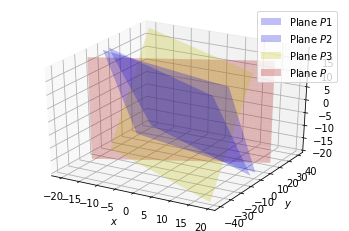
\includegraphics[ width=\columnwidth]{planes.png}
\caption{Plane $P$ passing through intersection of $P_{1}$ and $P_{2}$ and perpendicular to $P_{3}$}
\label{fig:Line }	
\end{figure}
\end{document}
